\section{When isolation is the stronger coordination mechanism}\label{sec:C21:isolation}
Consider two workers preparing changes to different modules of one repository. Their edits appear independent, but both modify a shared interface specification. A shared writable checkout permits immediate coordination through the filesystem, yet it also permits one worker to test a transient mixture of changes. The resulting passing test verdict may correspond to no committed artifact. A later merge can then fail despite both workers reporting success. This is an evidence-identity failure rather than a lack of programming ability.

An isolated-workspace design gives each worker a base revision and a separate branch. The manager merges their artifacts and runs integration checks on the merged digest. This adds storage and validation cost but creates a clear causal boundary: worker tests concern branch artifacts; integration tests concern the combined artifact. If the interface changes are incompatible, the conflict is explicit. Isolation does not prevent semantic incompatibility, but it prevents accidental shared state from concealing it.

The same reasoning applies to research. Two investigators can independently inspect conflicting papers before receiving each other's conclusions. Their private notes preserve the evidence that motivated each interpretation. Discussion then operates on the disagreement rather than on an already homogenized summary. Complete isolation would prevent useful correction, so the design uses staged disclosure: independent extraction first, evidence exchange second, joint interpretation third. The stages allow an experiment to observe where agreement arises.

For memory systems, isolation can be temporary and selective. A worker may read a shared evidence snapshot while writing candidate interpretations to a private namespace. A promotion gate checks provenance, conflicts, and applicability before moving those interpretations into shared memory. This resembles a database transaction but adds semantic evaluation. The gate can still make mistakes, and its acceptance threshold determines the tradeoff between contamination and delayed learning. Promotion should therefore retain the original candidate and gate verdict for later audit.

The cost of this mechanism grows with candidate volume. If every worker proposes many redundant records, verification can dominate execution. Deduplication before promotion reduces load, but semantic deduplication can incorrectly merge distinct conditions. A safer first stage deduplicates exact source identities and artifact hashes; a later stage considers whether two interpretations are equivalent under their stated scope. Keeping these stages separate makes it possible to attribute errors to retrieval, deduplication, or review.

An evaluation should compare immediate shared writes, snapshot reads with private writes, and fully isolated memory under the same task sequence. Inject one incorrect but plausible record and measure its propagation, subsequent correction, and effect on task outcomes. Also include a valid rare record: a system that blocks all unusual memories may contain contamination while preventing beneficial transfer. Measure both harmful propagation and useful adoption, along with the review work needed to distinguish them.

The implication is conditional rather than categorical. Shared state is valuable when its information benefits exceed its coordination and contamination costs. Isolation is valuable when it preserves evidence identity, authority boundaries, or independent judgment. A principal design decision is to choose the smallest shared surface required for the task. Increasing communication and memory visibility without identifying the dependency they serve is not a scientific explanation of why a team should improve.


Figure~\ref{fig:C21:overview} isolates the mechanism and its stated information boundaries.
\begin{figure}[!htbp]
\centering
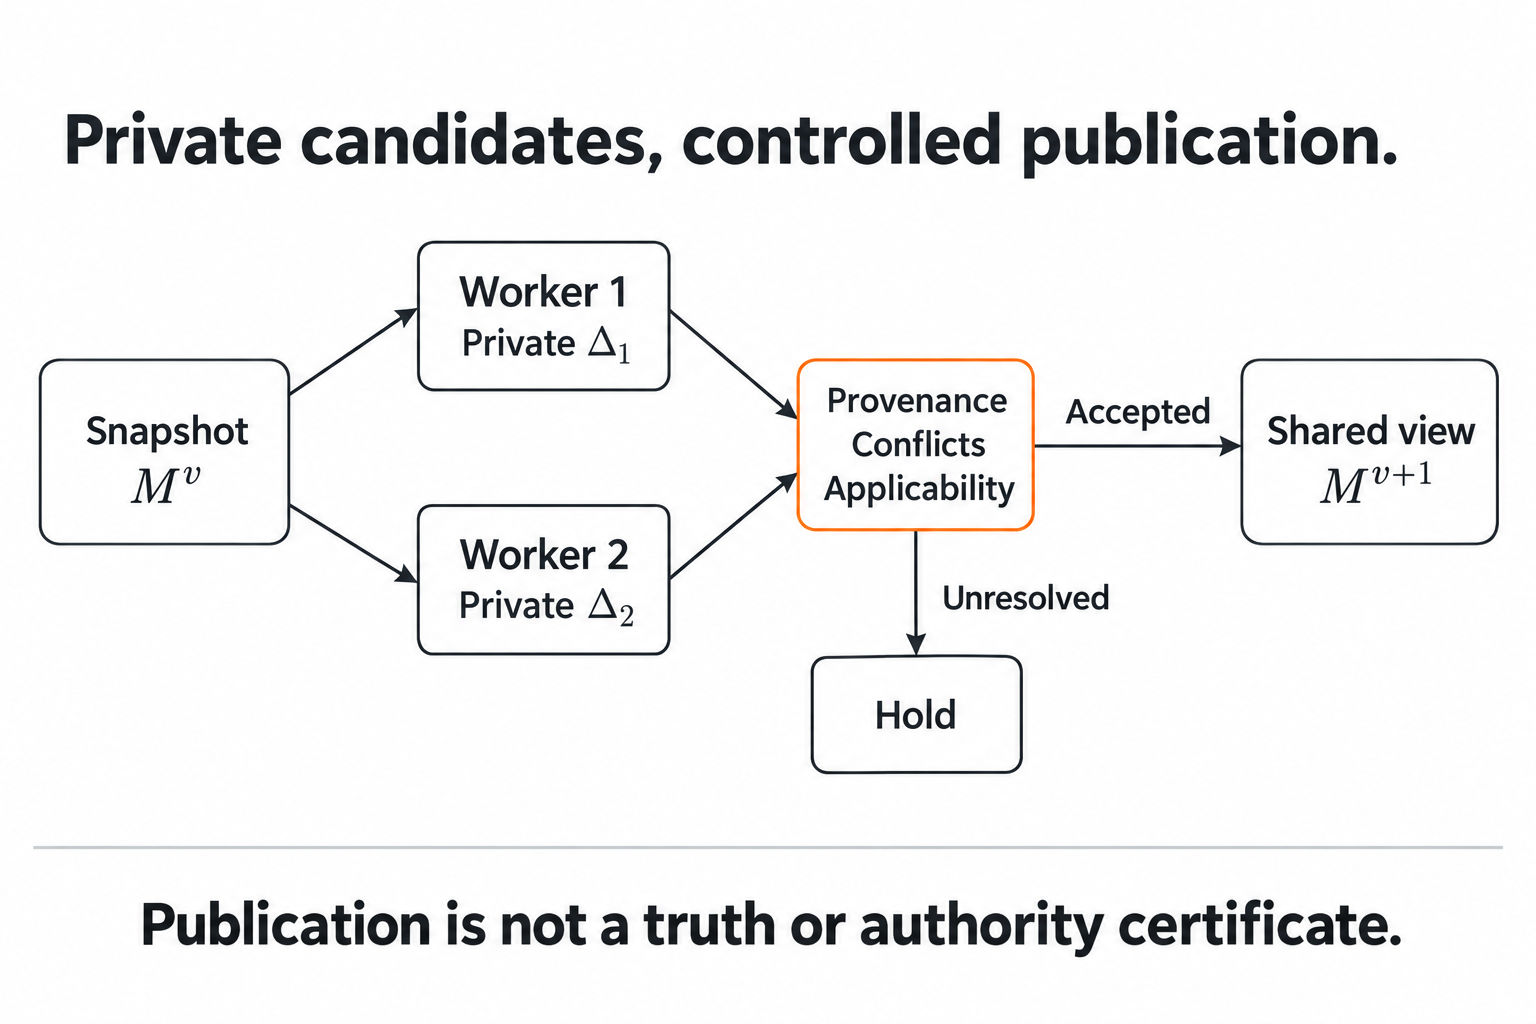
\includegraphics[width=\linewidth]{book/figures/assets/F21review.png}
\caption{Workers can read one versioned snapshot while retaining candidate interpretations privately. Only the promotion path publishes accepted candidates into a new shared view; unresolved candidates remain separate. Provenance, conflict and applicability checks retain an auditable decision boundary. The gate does not establish semantic truth, current effect authority, or a performance improvement.}
\label{fig:C21:overview}
\end{figure}
